\section{Model-Based Statistical Analysis} \label{sec:confirmatory}
Given the longitudinal nature of the study, in addition to considering the effect that the month and treatment variables have on reducing the level of mental distress across all participants, it is also important to address the correlation among the GSI scores obtained from each individual participant. The mixed-effects model is one of the most popular for analyzing longitudinal data for its intuitiveness and high interpretability. Particularly, it handles the individual-specific correlation by adding additional parameters at the individual level. Since the response (GSI) is continuous, and we have both continuous (month, education) and categorical (treatment, gender) explanatory variables, a natural model of choice is the linear mixed-effects model.\\\\
The linear mixed-effects model takes on the following general form:
\begin{align}
y_{ij} = (\beta_0 + b^0_i) + (\beta_1 + b^1_i)t_{ij} + (\beta_2 + b^2_i)x^2_i + \cdots + (\beta_n + b^n_i)x^n_i + e_{ij}. \label{eq:lme}
\end{align}
In our case, $y_{ij}$ denotes the GSI score of the $i$th participant at the $j$th time point. $t_{ij}$ represents the month variable for the $i$th participant at the $j$th time point. $x^2_i,\cdots,x^n_i$ correspond to the other explanatory variables that do not change over time for the $i$th participant. Finally the $e_{ij}$ terms are the residuals, which are assumed to be normally distributed and centred at $0$.\\\\
By fixing $j$ and ignoring the $b_i$ terms, we recover the familiar linear regression model, where the $\beta$ terms represent the effects of each explanatory variable on the response. By varying the time points $j$, we are able to model the effects of each explanatory variable considering the changes in the response over time. Including the $b_i$ terms allows the individual-specific correlation to be taken into consideration. The $b_i$ terms are the random effects. It is assumed that for each $k, b_i^k\sim N(0, \sigma^2_k)$ across all $i$.\\\\
Both of the questions that we would like to answer can be analyzed using different linear mixed-effects models. Specifically, by looking at the participants in the intervention group and the control group separately, the effect of the month variable on the GSI scores describes how mental distresses in each of the groups change over time. At the same time, by looking at both groups together, we can quantify the effect of mental health intervention by inspecting the $\beta$ term associated with the treatment variable. As a result, for the remainder of this section, we present in detail the analysis procedure that addresses whether mental distress decreases over time in the intervention group as an example. The analysis results addressing both of our main questions are carefully discussed in \cref{sec:analysis.results}.\\\\
Before proceeding to selecting the appropriate linear mixed-effects models that address our main objectives, it is worth noting that all of the entries that contain missing values, either on the explanatory variables or the response, are removed before conducting the following analysis. In addition, all of the participants with only one recorded GSI score are also excluded from the analysis below. This is because in such cases, there is no information on how the participant's mental distress has changed over time. Under the linear mixed-effects models, the removal of such observations implies that we are imposing the additional assumption that the reasons these values are missing do not depend on the missing values themselves. The missing values are more carefully treated in \cref{sec:handling.missing.data}.
\subsection{Model Selection}
\begin{wraptable}{r}{0.5\textwidth}
\resizebox{\linewidth}{!}{
\begin{tabular}{|l|l|l|}
\hline
& month & month/gender/education \\
\hline
month/gender & 0 & 0.016 \\
\hline
month/education & 0.004 & 0 \\
\hline
\end{tabular}
}
\caption{P values of Likelihood Ratio tests between models with different covariates under the intervention group}
\label{tab:model.comp.treatment.lrt}
\end{wraptable}
From \cref{eq:lme}, it is clear that setting any of the $\beta$'s to 0 implies the corresponding explanatory variable is not included in the linear mixed-effects model. At the same time, setting any set of $b_i^k$'s across all $i$ to 0 means that the random effects associated with the corresponding explanatory variable are not considered. A natural next step is then to identify the covariates and mixed effects that we would like to include in the model. By \cite{wu2009mixed}, common model selection metrics such as the AIC, BIC, and the p-values from likelihood ratio tests (LRT) can be employed. Both the AIC and BIC try to find the balance between goodness-of-fit and model complexity. In our case, since the total number of explanatory variables considered is not large, we are not overly concerned with model complexity. Therefore, we use the p-values from LRT to select an appropriate model to answer whether the mental distresses decrease over time among participants in the intervention group. The LRT tests whether one model is a significantly better fit than the other between two nested models. By nested models, we mean that the parameters of the smaller model form a subset of those of the larger model.\\\\
We begin by selecting the explanatory variables to be included in the model. Since we're interested in the changes of mental distress over time, the month variable must be included. From \cref{sec:eda}, we know that it is possible that one of the gender and education variables can explain much of the variabilities among the GSI scores. Therefore we compare the goodness-of-fit among models that include varying covariates using the LRT. The p-values are summarized in \cref{tab:model.comp.treatment.lrt}. Note that none of the mixed effects is considered here. In \cref{tab:model.comp.treatment.lrt}, the first column shows there is strong evidence (p-values $<0.004$) that including either of the gender or education variables leads to a better fit model. Then the second column shows there is moderate to strong evidence (p-values $<0.016$) including both covariates leads to a better fit model compared to those that only include one. As a result, we do not discard any of the covariates when studying the change in mental distress among participants in the intervention group. Similarly, as shown in \cref{app:cov.control,app:cov.both}, none of the covariates is discarded. Note that in \cref{app:cov.both}, the treatment variable is also included automatically because its effect is essential to detecting any effect of mental health intervention.\\
\begin{figure}[t]
\begin{subfigure}{.33\textwidth}
  \centering
  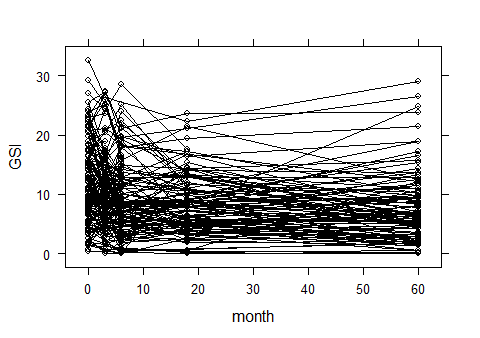
\includegraphics[width=1\linewidth]{../../plots/trellis_treatment.png}
  \caption{trellis plot of all subjects in the intervention group}
  \label{fig:4a}
\end{subfigure}
\begin{subfigure}{.33\textwidth}
  \centering
  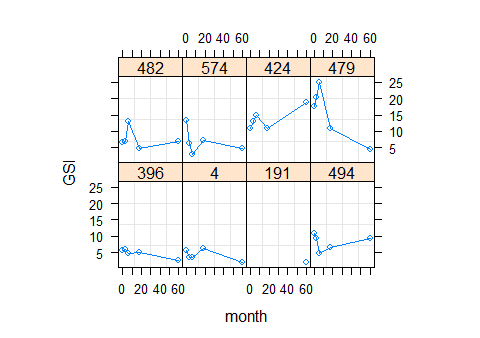
\includegraphics[width=1\linewidth]{../../plots/trellis_subset_treatment.png}
  \caption{trellis plot of randomly selected subjects}
  \label{fig:4b}
\end{subfigure}
\begin{subfigure}{.33\textwidth}
  \centering
  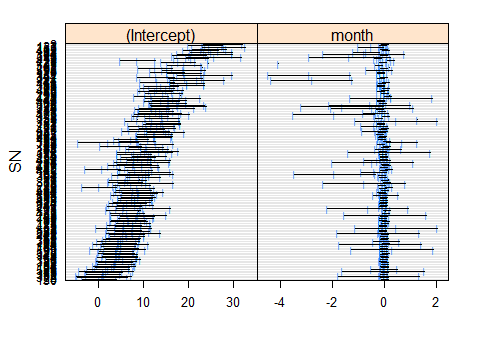
\includegraphics[width=1\linewidth]{../../plots/interval_treatment.png}
  \caption{confidence intervals of parameters from individual linear models}
  \label{fig:4c}
\end{subfigure}
\caption{Diagnostic plots for selection of random effects for the intervention group}
\label{fig:diagnostic.treatment}
\end{figure}

\noindent Now that the covariates to be included are determined for each model, the random effects can be selected following the same approach. The random effects allows us to adjust the effect that a explanatory variable or the intercept has for each participant on top of the overall average effect. Before formally deciding which random effects are to be included using the LRT, we use the plots in \cref{fig:diagnostic.treatment} to gauge whether the inclusion of any random effects is warranted.\\
\begin{wraptable}{r}{0.5\textwidth}
\resizebox{\linewidth}{!}{
\begin{tabular}{|l|l|l|l|}
\hline
& no mixed effect & intercept & intercept/month \\
\hline
intercept & 0 &/ &/ \\
\hline
intercept/month &/ & 0.028 &/ \\
\hline
intercept/gender &/ & 0.784 &/ \\
\hline
intercept/education &/ & 0.998 &/ \\
\hline
intercept/month/gender & /&/ & 0.893 \\
\hline
intercept/month/education & /&/ & 0.995 \\
\hline
\end{tabular}
}
\caption{P values of Likelihood Ratio tests between models with different mixed effects under the intervention group}
\label{tab:model.comp.treatment.me.lrt}
\end{wraptable}
\noindent By \cref{fig:4a}, it is clear that at the beginning of the study, the participants' levels of mental distresses are quite different in the intervention group. To better assess how the GSI scores change over time, we randomly select some of the participants and show how their GSI scores change over the course of the study in \cref{fig:4b}. While many of the participants' GSI scores exhibit an overall flat trend, there are participants whose GSI scores show clear increasing or decreasing trends acorss time. To better access the trends across time among all participants in the intervention group, we fit linear regression models without random effects on each of the participants' GSI scores individually and plot the 95\% confidence intervals of the regression parameters in \cref{fig:4c}. This plot verifies the variability present in the GSI scores at the beginning of the study as many of the confidence intervals of the individual intercepts do not overlap. While most confidence intervals of the individual regression parameters for the month variable hover around 0, we do have two instances where the confidence intervals are much different than the rest. These plots suggest that a random effect term is necessary for both the intercept and the month variable.\\\\
It is important to note, though, that each participant's gender and education variables do not change over the course of the study. Therefore when fitting individual linear regression models on each of the participants, the effect of the gender and education variables cannot be distinguished from the intercept. As a result, we only know that a random effect term is necessary for some of the intercept and the gender and education variables. To formally decide where to place the random effects among the intercept and the two covariates, we again use the p-values from the LRT.\\\\
As shown in \cref{tab:model.comp.treatment.me.lrt}, a stepwise procedure is used when comparing models that contain different random effect terms. We first note that adding a random effect term on the intercept leads to better fit model (p-value $\approx 0$). Then among the three covariates, there is moderate evidence that adding a random effect on the month variable leads to a better fit (p-value = 0.028). Finally, there is no evidence against that further including random effects on either gender or education results in the same level of goodness-of-fit (p-values $>0.893$). Therefore, when studying the changes in mental distress over time in the intervention group, a model that includes random effects on the intercept and the month variable is most appropriate.\\\\
Following the same procedure, as shown in \cref{app:re.control}, a random effect term is only added to the intercept term when studying the changes in mental distress over time in the control group. In \cref{app:re.both}, we see that random effect terms are added to both the intercept and the month variable.
\subsection{Assumption Check}

\begin{figure}[H]
\centering
\begin{subfigure}{.4\textwidth}
  \centering
  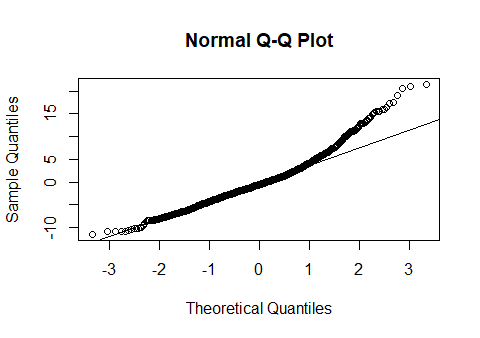
\includegraphics[width=1\linewidth]{../../plots/qq_residual_treatment.png}
  \caption{residual QQ plot}
\end{subfigure}
\begin{subfigure}{.4\textwidth}
  \centering
  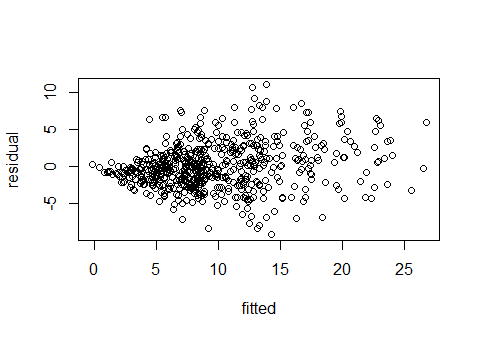
\includegraphics[width=1\linewidth]{../../plots/residual_treatment.png}
  \caption{fitted value vs. residual (t-test: 1, Wilcoxon: 0.204)}
\end{subfigure}
\caption{Visualizing the residuals of the LME model under the intervention group}
\label{fig:residual.treatment}
\end{figure}

\begin{figure}[H]
\centering
\begin{subfigure}{.4\textwidth}
  \centering
  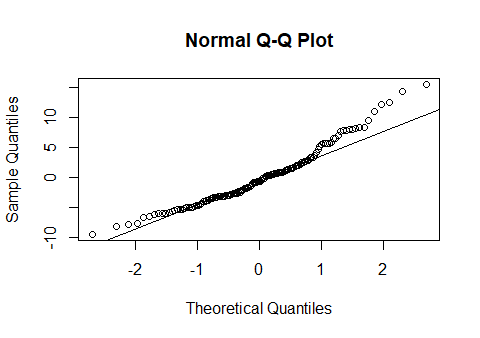
\includegraphics[width=1\linewidth]{../../plots/qq_intercept_treatment.png}
  \caption{QQ plot for the random effects on the intercept (t-test: 1, Wilcoxon: 0.335)}
\end{subfigure}
\begin{subfigure}{.4\textwidth}
  \centering
  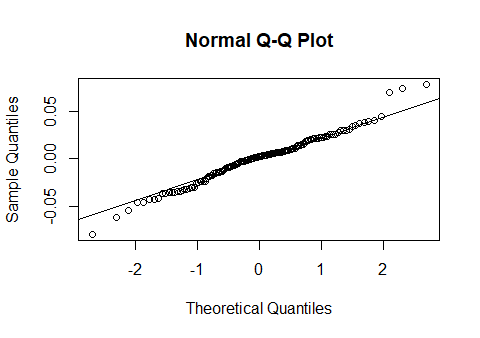
\includegraphics[width=1\linewidth]{../../plots/qq_slope_treatment.png}
  \caption{QQ plot for the random effects on the slope (t-test: 1, Wilcoxon: 0.781)}
\end{subfigure}
\caption{Visualizing the random effects under the intervention group}
\label{fig:re.treatment}
\end{figure}

\subsection{Analysis results}\label{sec:analysis.results}
\subsubsection{Changes in Mental Distress over Time}
\begin{table}[H]
\begin{minipage}{0.5\textwidth}
\centering
\resizebox{\linewidth}{!}{
\begin{tabular}{|l|r|r|r|r|r|}
\hline
  & Value & Std.Error & DF & t-value & p-value\\
\hline
(Intercept) & 11.933 & 2.758 & 465 & 4.326 & 0.000\\
\hline
month & -0.047 & 0.008 & 465 & -5.671 & 0.000\\
\hline
gender2 & 2.764 & 0.925 & 141 & 2.990 & 0.003\\
\hline
education & -0.249 & 0.190 & 141 & -1.314 & 0.191\\
\hline
\end{tabular}
}
\caption{Output of Linear Mixed Model under the intervention group}
\label{tab:lme.treatment}
\end{minipage}
\hfill
\begin{minipage}{0.5\textwidth}
\centering
\resizebox{\linewidth}{!}{
\begin{tabular}{|l|r|r|r|r|r|}
\hline
  & Estimate & Naive S.E. & Naive z & Robust S.E. & Robust z\\
\hline
(Intercept) & 11.162 & 2.484 & 4.494 & 2.538 & 4.397\\
\hline
month & -0.047 & 0.010 & -4.477 & 0.008 & -5.852\\
\hline
gender2 & 2.827 & 0.834 & 3.391 & 0.869 & 3.253\\
\hline
education & -0.194 & 0.170 & -1.146 & 0.173 & -1.125\\
\hline
\end{tabular}
}
\caption{Output of GEE model under the intervention group}
\label{tab:gee.treatment}
\end{minipage}
\end{table}

\begin{table}[H]
\begin{minipage}{0.5\textwidth}
\centering
\resizebox{\linewidth}{!}{
\begin{tabular}{|l|r|r|r|r|r|}
\hline
  & Value & Std.Error & DF & t-value & p-value\\
\hline
(Intercept) & 19.235 & 4.151 & 308 & 4.634 & 0.000\\
\hline
month & -0.020 & 0.008 & 308 & -2.394 & 0.017\\
\hline
gender2 & 2.606 & 1.383 & 95 & 1.884 & 0.063\\
\hline
education & -0.822 & 0.273 & 95 & -3.015 & 0.003\\
\hline
\end{tabular}
}
\caption{Output of Linear Mixed Model under the control group}
\label{tab:lme.control}
\end{minipage}
\hfill
\begin{minipage}{0.5\textwidth}
\centering
\resizebox{\linewidth}{!}{
\begin{tabular}{|l|r|r|r|r|r|}
\hline
  & Estimate & Naive S.E. & Naive z & Robust S.E. & Robust z\\
\hline
(Intercept) & 19.267 & 3.433 & 5.613 & 3.229 & 5.967\\
\hline
month & -0.027 & 0.013 & -2.019 & 0.010 & -2.606\\
\hline
gender2 & 2.220 & 1.148 & 1.935 & 1.216 & 1.825\\
\hline
education & -0.809 & 0.225 & -3.596 & 0.203 & -3.994\\
\hline
\end{tabular}
}
\caption{Output of GEE model under the control group}
\label{tab:gee.control}
\end{minipage}
\end{table}

\subsubsection{Effectiveness of Mental Health Intervention}

\begin{table}[H]
\begin{minipage}{0.5\textwidth}
\centering
\resizebox{\linewidth}{!}{
\begin{tabular}{|l|r|r|r|r|r|}
\hline
  & Value & Std.Error & DF & t-value & p-value\\
\hline
(Intercept) & 15.418 & 2.341 & 774 & 6.586 & 0.000\\
\hline
treatment2 & -0.193 & 0.731 & 238 & -0.264 & 0.792\\
\hline
month & -0.037 & 0.006 & 774 & -5.893 & 0.000\\
\hline
gender2 & 2.737 & 0.776 & 238 & 3.527 & 0.001\\
\hline
education & -0.516 & 0.157 & 238 & -3.295 & 0.001\\
\hline
\end{tabular}
}
\caption{Output of Linear Mixed Model}
\label{tab:lme}
\end{minipage}
\hfill
\begin{minipage}{0.5\textwidth}
\centering
\resizebox{\linewidth}{!}{
\begin{tabular}{|l|r|r|r|r|r|}
\hline
  & Estimate & Naive S.E. & Naive z & Robust S.E. & Robust z\\
\hline
(Intercept) & 14.685 & 2.046 & 7.176 & 2.053 & 7.154\\
\hline
treatment2 & -0.430 & 0.641 & -0.671 & 0.735 & -0.586\\
\hline
month & -0.039 & 0.008 & -4.666 & 0.006 & -6.040\\
\hline
gender2 & 2.693 & 0.680 & 3.961 & 0.716 & 3.763\\
\hline
education & -0.455 & 0.136 & -3.337 & 0.139 & -3.278\\
\hline
\end{tabular}
}
\caption{Output of GEE model}
\label{tab:gee}
\end{minipage}
\end{table}

\subsection{Handling Missing Data} \label{sec:handling.missing.data}
\cite{little2019statistical}